%-----------------------------------------------------------------
%	TOOLS AND DATA
%	!TEX root = ./../main.tex
%-----------------------------------------------------------------
\section[The N Queens Problem]{The $N$ Queens Problem}\label{sec:problem}\nocite{Pearl1984}
This problem consists on placing $N$ queens on a $N \times N$ chessboard so that no queen can attack another. In the usual fashion, an attack is defined when two or more queens are in the same row, column, or diagonal (as depicted in figure \ref{fig:4queens}). We will expand on how to compute if a queen attacks another in \cref{sec:fitness}.

\begin{figure}[H]
	\centering
	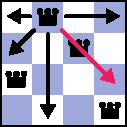
\includegraphics[height=0.18\textwidth]{4queens}
	\caption{Example of a queen attacking another queen on a $4 \times 4$ board}
	\label{fig:4queens}
\end{figure}

The problem can be quite expensive from a computational point of view, as there are $N^{N}$ possible arrangements of $N$ queens on an $N \times N$ board, but only a small amount of solutions (relative to the total possible arrangements). It is possible, however, to use shortcuts that reduce computational requirements of brute-force techniques.

\subsection{Computational representation}\label{sec:representation}
Given the nature of this problem, we can program our algorithm to work with queens so that no queen shares the same row or column. The simplest way is to think of each board as an array of non-repeated consecutive numbers, where the index represents the row, and the number itself is the column; this is called \emph{Permutation Representation}. For instance, the board in figure \ref{fig:4queens} would be represented as
\begin{align}
	\inline{[1 2 0 3]}.
\end{align}

This consideration alone makes the complexity of a brute-force algorithm much simpler, as now we only have $N!$ possible permutations of $N$ queens on an $N \times N$ board (we will expand on this later).

%-----------------------------------------------------------------
\subsection{Solutions of the problem}

Table \ref{tab:all-sols} summarises the number of solutions for the $N$ Queens Problem, both fundamental and all (or non-fundamental) solutions, where fundamental solutions are those that exclude mirrored images as well as rotations of a solution.

There is currently no known formula for the exact number of solutions, or even for its asymptotic behaviour for larger values of $N$.
\begin{table}[H]
	\centering
	\begin{tabular}{r | ccccccccccc}
		\toprule
		\toprule
		$N$         & 1 & 2 & 3 & 4 & 5 & 6 & 7 & 8 & 9 & 10 & ... \\
		\midrule
		fundamental & 1 & 0 & 0 & 1 & 2 & 1 & 6 & 12 & 46 & 92 & ... \\
		all         & 1 & 0 & 0 & 2 & 10 & 4 & 40 & 92 & 352 & 724 & ... \\
		\bottomrule
	\end{tabular}
	\caption{List of solutions for the $N$ Queens Problem}
	\label{tab:all-sols}
\end{table}

All non-fundamental solutions up to $N = 10$ can be easily obtained using the script \inline{brute-queens.py}. We will not discuss the details of the implementation, for it is a really simple algorithm, and brute-force methods are not the main focus of this text.

As an illustration, in figure \ref{fig:4queens-sols} we depict the only two non-fundamental solutions for $N = 4$. It is worth to notice that the two solutions are the same fundamental solution, as they are the mirrored image of each other.

\begin{figure}[H]
	\centering
	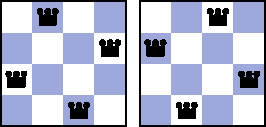
\includegraphics[height=0.18\textwidth]{4queens-sols}
	\caption{The two non-fundamental solutions of the 4 Queens Problem}
	\label{fig:4queens-sols}
\end{figure}

In figure \ref{fig:queens-sols} we compare the complexity of using an algorithm that calculates all possible arrangements and another that only calculates all the possible permutations against the amount of non-fundamental solutions for the $N$ Queens Problem.
\begin{figure}[H]
	\centering
	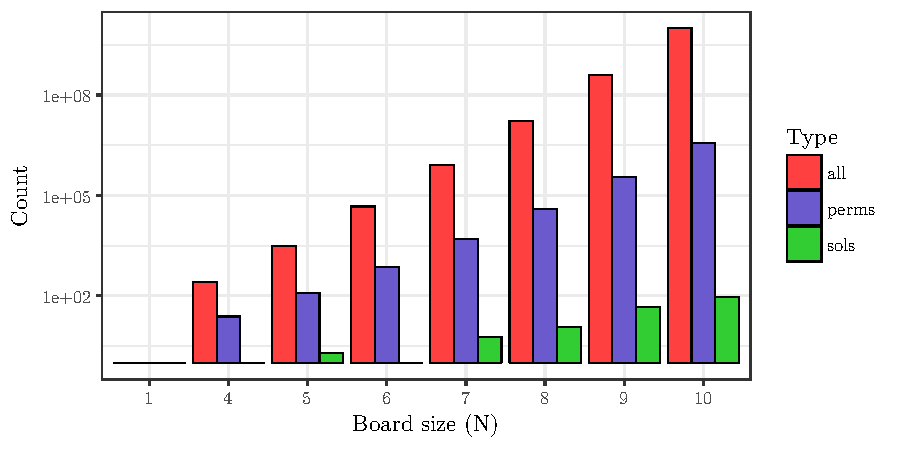
\includegraphics[width=0.95\textwidth]{queens-sols}
	\caption{Comparison of brute-force complexity for the $N$ Queens Problem}
	\label{fig:queens-sols}
\end{figure}

%-----------------------------------------------------------------
\subsection{Role of metaheuristics}
One may think that using only permutations gives us a good enough brute-force method to solve this problem. This may be true for small values of $N$, but $N > 10$ presents quite a computational barrier in terms of memory requirements. Using $N = 11$ requires calculating $11! = \num{39916800}$ different permutations; this means using $\sim \SI{3.5}{GB}$ of RAM\footnote{On a 64-bit platform (8 bits per integer).} just to store the numbers on the boards (the boards' structure would be another thing altogether).

It is for this reason that heuristics are used to solve this kind of problem, as they can be used to speed up the process of finding a solution. In particular, we will solve the $N$ Queens Problem using a Genetic Algorithm, a metaheuristic inspired by the process of natural selection that belongs to the larger class of evolutionary algorithms. We will discuss this implementation in \cref{sec:implementation}.



